\documentclass[12pt,titlepage]{article}

% This first part of the file is called the PREAMBLE. It includes
% customizations and command definitions. The preamble is everything
% between \documentclass and \begin{document}.

\usepackage[margin=1in]{geometry}  	% set the margins to 1in on all sides
\usepackage{setspace} \doublespacing 	% double spaced
\usepackage{graphicx}              			% to include figures
\usepackage{subcaption}				% to use sub captions
\usepackage{epstopdf}
\usepackage{amsmath}               		% great math stuff
\usepackage{amsfonts}              		% for blackboard bold, etc
\usepackage{amsthm}                		% better theorem environments
\usepackage[numbers]{natbib}			% for bibiliography with numbers
\usepackage{hyperref}				% make link clickable


%%%%%%%%%%%%%%%%%%%%%%%%
% Document Begins Here %
%%%%%%%%%%%%%%%%%%%%%%%%

\begin{document}

\begin{titlepage}
    \begin{center}
        \vspace*{1cm}


        {\scshape\Large CMPUT681\par}
        {\scshape\LARGE Parallel and Distributed Systems\par}   
        \vspace{0.5cm}
        {\scshape\Large Project Report - Fall 2022\par}
        \vfill
        
        %%%% PROJECT TITLE
        \Huge
        \textbf{The eXpress Data Path\\}
        \LARGE
        Fast Programmable Packet Processing in the Operating System Kernel

        \vfill

        %%%% AUTHOR(S)
        {\Large Naveenraj Muthuraj\par}
        {\Large nmuthura@ualberta.ca \par}
        {\Large 1769237 \par}

    \end{center}
\end{titlepage}

\doublespacing
\tableofcontents
\singlespacing

\newpage

\doublespacing


\section{Introduction}

Network stacks in general purpose operating systems are typically optimised for flexibility. 
This means they perform too many operations per packet, this will eventually lead to bottleneck in network performance  since the network devices and interfaces nowadays come with high speed packets rates upto 100Gbps . This has led to the increasing popularity of software packet processing, such as Data Plane Development Kit (DPDK) \cite{dpdk}. These tools are implemented using kernel bypass techniques, where a userspace application takes complete control of the networking hardware to avoid expensive context switch between kernel and userspace. 

While the kernel bypass approach can significantly improve performance it has its own drawbacks. Firstly, It is difficult to integrate with existing system. Secondly the applications have to re-implement functionality otherwise provided by the operating system network stack, 
such as routing tables and higher level protocols. Lastly, userspace application implementing entire networking stack will increase complexity and blurs security boundaries otherwise enforced by the operating system kernel. 

To overcome these drawbacks of kernel bypass design. \citet{xdp} presented a system that adds programmability directly in the operating system networking stack in a cooperative way. This makes it possible to perform high-speed packet processing that integrates seamlessly with existing systems, while selectively leveraging functionality in the operating system. This framework, is called the eXpress Data path (XDP). 

In this report we present a brief introduction to XDP and the results of reproducing the experiments originally conducted by \citet*{xdp}, which shall be referred to has the \textit{original paper} throughout this report.
This is structured as follows: Section 2 brief note on XDP, Section 3 experiment setup and Section 4 presents performance evaluation in comparison to original study and Section 5 Illustrates the use of XDP in real-world use cases and its performance graphs. Section 6 concludes.

\section{The XDP}

eXpress Data Path (XDP) works by defining a limited execution environment in the form of a virtual machine running eBPF code, an extended version of original BSD Packet Filter(BPF) \cite{mccanne_bsd_1993} byte code format.  The BPF environment executes eBPF programs (custom code) in the kernel space, before the kernel itself touches the packet data. Hence allowing packet processing at the earliest possible point after a packet is received from the network interface. The safety of the custom eBPF code is guaranteed  by The eBPF verifier. 

XDP which first got merged into the Linux kernel at version 4.8 , has since been actively developed and adopted across the industry. To name a few, Cloudflare uses XDP for their Distributed Denial of Service (DDoS) Mitigation \cite{cloudflare-ddos} and Facebook uses XDP in their Katran \cite{katran} project which is used for  Layer 4 Load-Balancing at scale. The vast applications of eXpress Data Path (XDP) and the eBPF virtual machine in the field of networking and observability is growing rapidly,  as Cloudflare engineer rightly puts it \textit{``eBPF  eats the world"}\footnote{\href{https://blog.cloudflare.com/cloudflare-architecture-and-how-bpf-eats-the-world/}{Cloudflare - How eBPF eats the world}} 


\section{Experiments}

All Experiment setup and implementation details is used from the \textit{original paper's} artifact \cite{xdp-test-data} . There are two major differences to this report's experiment a) Cloud based instances with virtual Network Interface card (NIC) is used and b) The performance evaluation is done on the latest stable Linux kernel version 5.15 . To reduce cost and make the experiments highly reproducible  the setup was fully automated using infrastructure as a code tool called Terraform \cite{terra}. Full details of our setup and scripts along with test data is made available in an online repository \cite{xdp-exp}.


\subsection{Experiment Setup}

The RFC 2544 \cite{rfc2544} for Network benchmarking was used as experiment setup as show in the Figure ~\ref{fig:setup}. The Cisco TRex \cite{cisco18:_trex_traff_gener} was used as traffic generator while the device under test (DUT) runs Ubuntu 22.04 with Linux kernel 5.15 and with XDP programs loaded. 

\begin{figure}[h]
\centering
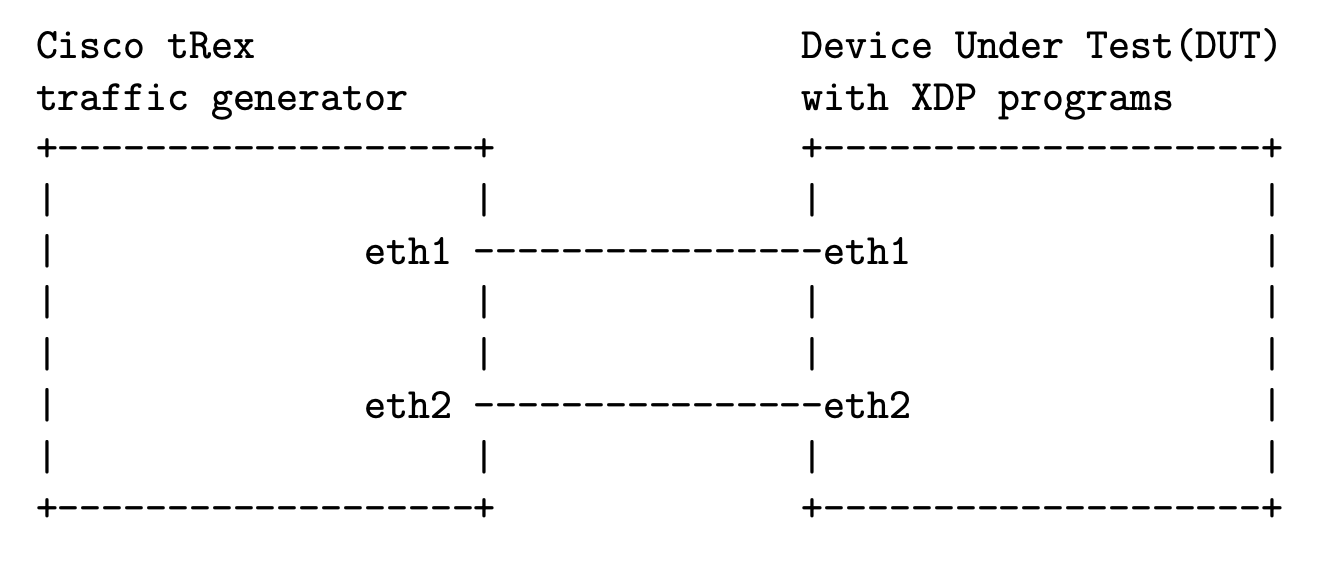
\includegraphics[width=0.8\textwidth]{img/exp_setup.png} 
\caption{RFC 2544 Experiment Setup }
\label{fig:setup}
\end{figure}


\subsection{Considerations}

From the initial analysis it was clear that to see any difference between Linux network stack and XDP, experiment should be conducted at higher packer per second (PPS) environment. Hence, the VMs in the local machine with maximum throughput of 1Gbps were deemed not suitable. To procure a NIC capable of 100Gbps speed an approximate cost would be around 2000 USD. Hence, We turned to cloud to avoid spending huge amount of money for NIC and finally decided to go with AWS. It is the only cloud provider which promises to provide near 100Gbps of speed. Table~\ref{tab:aws-table} shows network optimised EC2 instance of AWS. Even though the largest available instance c5n.18xlarge was used , we were not able to reach 100Gbps due to limitation of virtual instance , which is explained in the next section.

\begin{table}[]
\begin{tabular}{|l|r|r|r|r|l|}
\hline
\textbf{Instance Type} & \multicolumn{1}{l|}{\textbf{NIC}} & \multicolumn{1}{l|}{\textbf{NIC Queues}} & \multicolumn{1}{l|}{\textbf{CPU}} & \multicolumn{1}{l|}{\textbf{Memory}} & \textbf{Network Bandwidth} \\ \hline
\textit{c5n.large}     & 3                                 & 2                                        & 2                                 & 5.25                                 & Up to 25 Gigabit           \\ \hline
\textit{c5n.xlarge}    & 4                                 & 4                                        & 4                                 & 10.5                                 & Up to 25 Gigabit           \\ \hline
\textit{c5n.2xlarge}   & 4                                 & 8                                        & 8                                 & 21                                   & Up to 25 Gigabit           \\ \hline
\textit{c5n.4xlarge}   & 8                                 & 16                                       & 16                                & 42                                   & Up to 25 Gigabit           \\ \hline
\textit{c5n.9xlarge}   & 8                                 & 32                                       & 36                                & 96                                   & 50 Gigabit                 \\ \hline
\textit{c5n.18xlarge}  & 15                                & 32                                       & 72                                & 192                                  & 100 Gigabit                \\ \hline
\end{tabular}
\caption{AWS Network Optimised Instances and their Network Specifications}
\label{tab:aws-table}
\end{table}


\subsection{Limitations}

AWS EC2 Instances come with Elastic Network Interface(ENA) which is actually a PCIe Virtual Function, and the real link is actually the share physical network port. Due to this there were limitation which caused some difference between our setup and the original paper's setup. Example,  ENA does not support full Receive Side Scaling (RSS). Because of which we were unable to steer traffic to specific NIC RXs queues and hence to specific CPU. Due to this all experiments were only done with maximum 10 million PPS whereas the authors of original paper with physical Mellanox NIC operated at 100 million PPS. 

These experiments at lower PPS still serve the benefit to understand the impact of XDP at lower speeds.
The following experiments from the \textit{original paper} were left out of this study, due to resource constriants and technical difficulties. 
\begin{itemize}
  \item The DPDK performance comparison with XDP and Linux.
  \item Facebook Katran Load-Balancer performance evaluation. 
\end{itemize}


\section{Performance Evaluation}

The first graph in all the figures is from the \textit{original paper} which is used to compare our experiment results. 
For example, Figure~\ref{graph:xdp-drop:a} is from the \textit{original paper} whereas Figure~\ref{graph:xdp-drop:b} is the result of our experiments. The same is true for all subsequent figures.


\subsection{Packet Drop Performance}


Figure~\ref{graph:xdp-drop:b} shows the packet drop performance as a function of the number of cores. The baseline performance of XDP for a single core is just below 2 Mpps, while for Linux it is 1.1 Mpps. Two configuration of Linux network stack is measured. one is ``raw" table of iptables firewall module, which ensures the earliest possible drop in network stack; and another is conntrack module, which carries overhead as it tracks the network connection. By comparing with Figure~\ref{graph:xdp-drop:a}, we can say that the XDP performance really starts to differentiate with Linux at speed above 20 Mpps which we were not able to produce. Also it is clear that Linux conntrack module has high overhead even at lower PPS. Both Linux and XDP packet processing scales almost linearly with increase in number of cores. This is because as number of cores increases, the number of receive queues(RXs) per NIC also increases.

\begin{figure}
    \centering
    \begin{minipage}{0.49\textwidth}
        \centering
        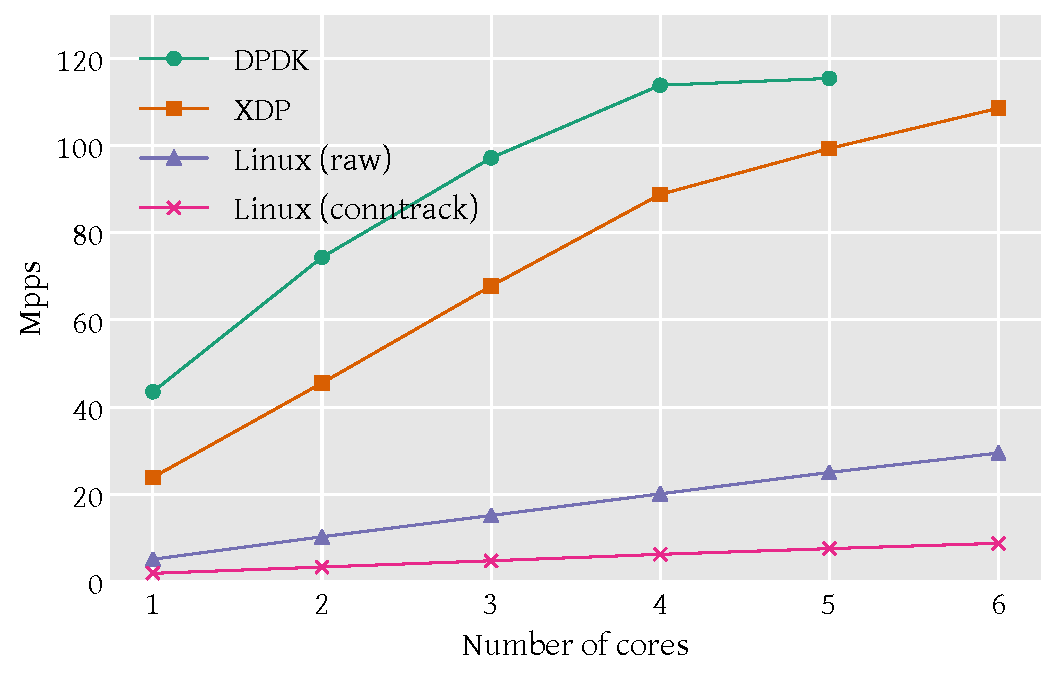
\includegraphics[width=0.95\textwidth,height=5.5cm]{original/drop-test.pdf} % first figure itself
        \subcaption{Packet drop performance in Higher PPS}
        \label{graph:xdp-drop:a}
    \end{minipage}\hfill
    \begin{minipage}{0.49\textwidth}
        \centering
        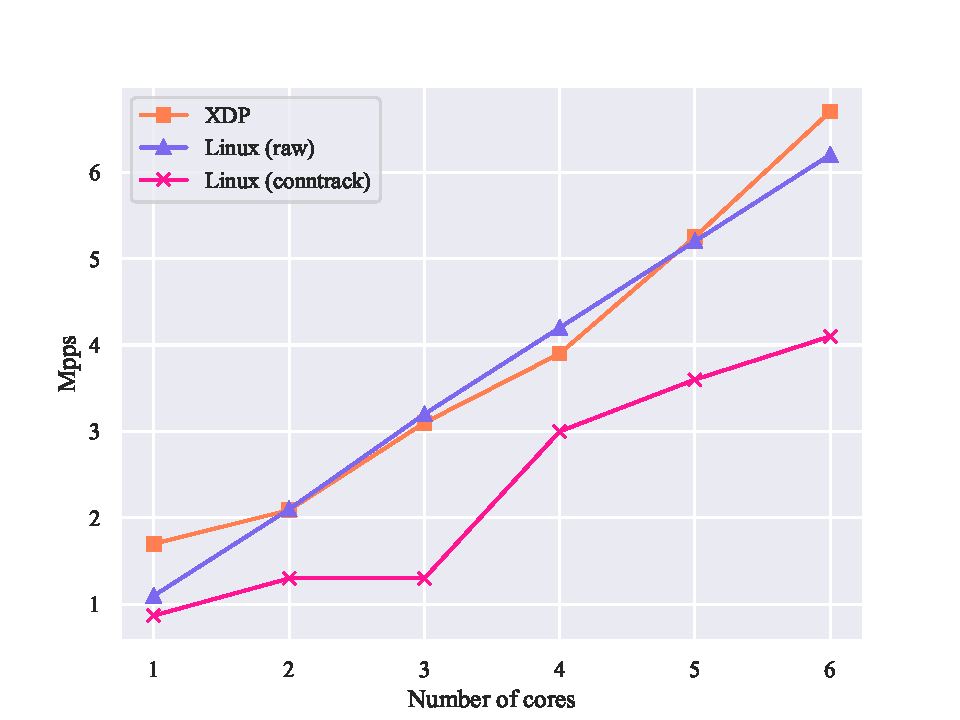
\includegraphics[width=0.95\textwidth,height=5.5cm]{img/drop-test.pdf} % second figure itself
        \subcaption{Packet drop performance in Lower PPS.}
        \label{graph:xdp-drop:b}
    \end{minipage}
     \caption{Packet drop performance.}
     \label{graph:xdp-drop}
\end{figure}

\subsection{CPU Usage}

CPU usage of the system was measured using \texttt{mpstat} while the packet drop application was running on a single CPU core. Figure~\ref{graph:drop-cpu:b} is very similar to Figure~\ref{graph:drop-cpu:a} showing that the XDP utilised less CPU in-comparison to Linux. The utilisation of both system increased as the load increases. However Linux stack reached close to  100\% utilisation quickly around 2 Mpps , but XDP showed smaller increase in CPU usage . We were not able to produce traffic in ourt setup to reach maximum CPU usage for XDP.

\begin{figure}
    \centering
    \begin{minipage}{0.49\textwidth}
        \centering
        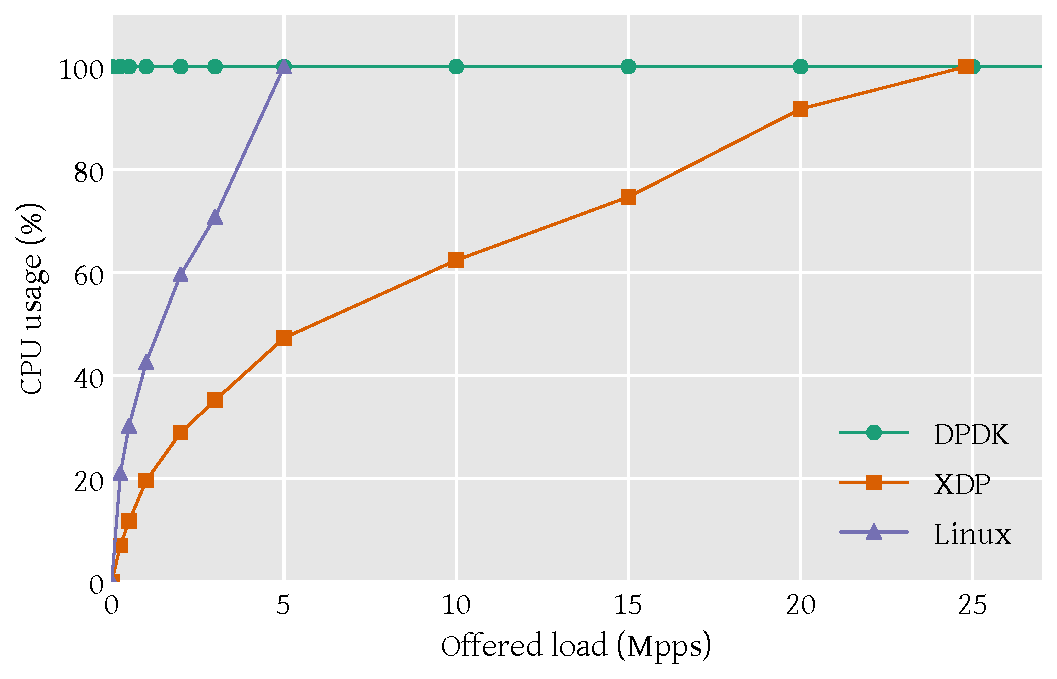
\includegraphics[width=0.95\textwidth,height=5.5cm]{original/drop-cpu.pdf} % first figure itself
        \subcaption{CPU usage in Higher PPS}
        \label{graph:drop-cpu:a}
    \end{minipage}\hfill
    \begin{minipage}{0.49\textwidth}
        \centering
        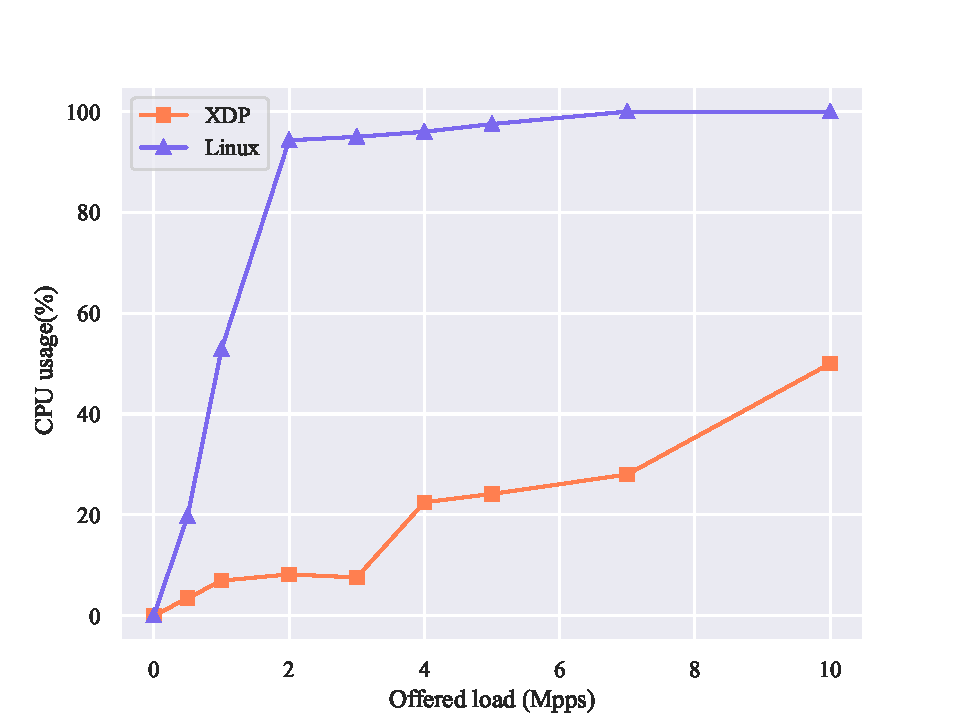
\includegraphics[width=0.95\textwidth,height=5.5cm]{img/drop-cpu.pdf} % second figure itself
        \subcaption{CPU usage in Lower PPS.}
        \label{graph:drop-cpu:b}
    \end{minipage}
     \caption{CPU usage in the drop scenario.}
     \label{graph:drop-cpu}
\end{figure}



\subsection{Packet Forwarding Performance}

Packet forwarding application simply swaps MAC address and forwards the packet either through same interface or different interface than the one it received through. Linux networking stack does not support minimal forwarding, but required full routing to forward packet. This is a expensive operation, since XDP doesn't perform this kind of operation. Linux comparison is left out and same is done in routing comparison. Figure~\ref{graph:redirect:b} shows packet forwarding performance of XDP system for same NIC and different NIC. Initially both same and different NIC forwarding have similar performance. This starts to change after around 3 Mpps.  Figure~\ref{graph:redirect:a} makes it evident that the difference in performance is much larger at higher PPS

\begin{figure}
    \centering
    \begin{minipage}{0.49\textwidth}
        \centering
        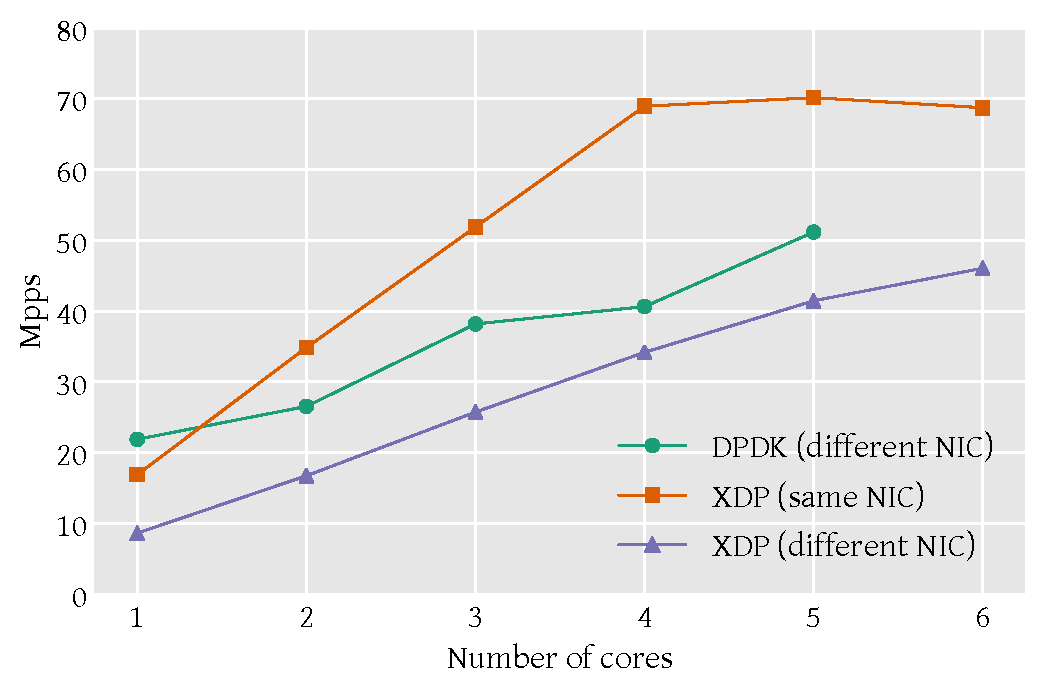
\includegraphics[width=0.95\textwidth,height=5.5cm]{original/redirect-test.pdf} % first figure itself
        \subcaption{throughput in Higher PPS}
        \label{graph:redirect:a}
    \end{minipage}\hfill
    \begin{minipage}{0.49\textwidth}
        \centering
        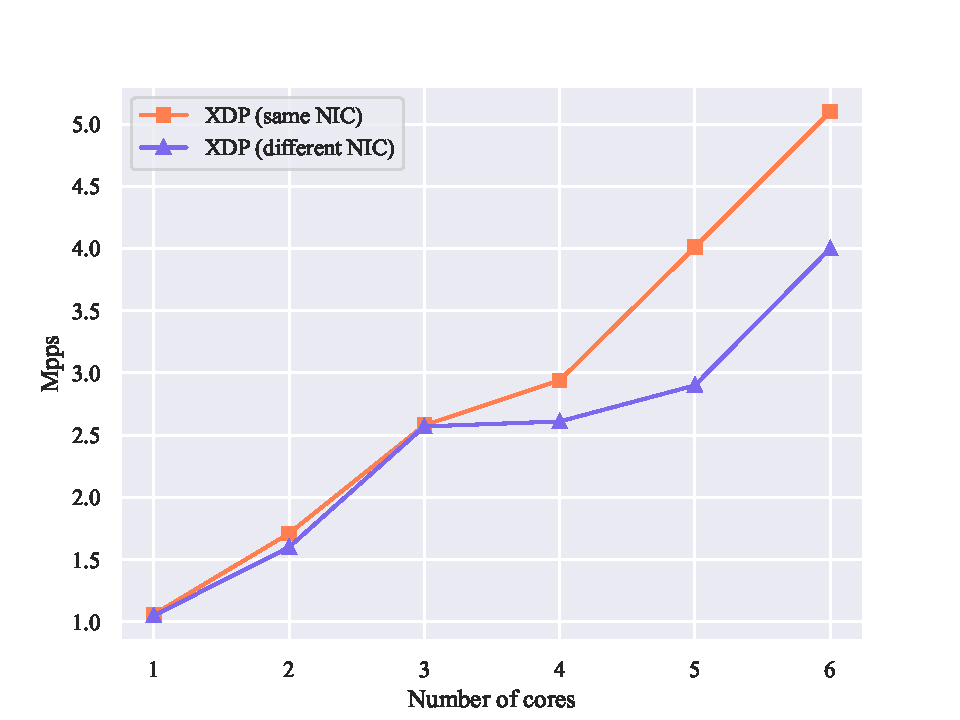
\includegraphics[width=0.95\textwidth,height=5.5cm]{img/redirect-test.pdf} % second figure itself
        \subcaption{throughput in Lower PPS.}
        \label{graph:redirect:b}
    \end{minipage}
     \caption{Packet forwarding throughput}
     \label{graph:redirect}
\end{figure}


\section{Real-world use cases}

To show how XDP can be used to implement useful real-world applications. Two experiments are performed,XDP in  traditional routing and inline Denial of Service (DoS) mitigation application.  

\subsection{Software Routing}

Linux kernel contains  a full-featured routing table. XDP is a natural fit for routing task, especially as it includes a helper function which performs full routing table lookups directly from XDP.

To show the performance of this XDP routing, we use XDP routing example that is included in Linux kernel source \cite{fwd-example} and compare its performance to routing using the regular Linux network stack.
We have omitted the full routing test done in  \textit{original paper} due to AWS VPC issues. The next-hop address in DUT is set to the address of the traffic generator system connected to our egress interface. So a packet going from traffic generator will hit the ingress interface of DUT and return back via egress interface. 

The Figure ~\ref{graph:route:b} shows the performance of XDP and Linux routing for a route table with single entry. Using XDP for the forwarding plane improves performance with a factor of 3. Which is consistent with the results of \textit{original} experiment ~\ref{graph:route:b}. This means a software router with XDP can perform much better routing than Linux using a single core.

\begin{figure}
    \centering
    \begin{minipage}{0.7\textwidth}
        \centering
        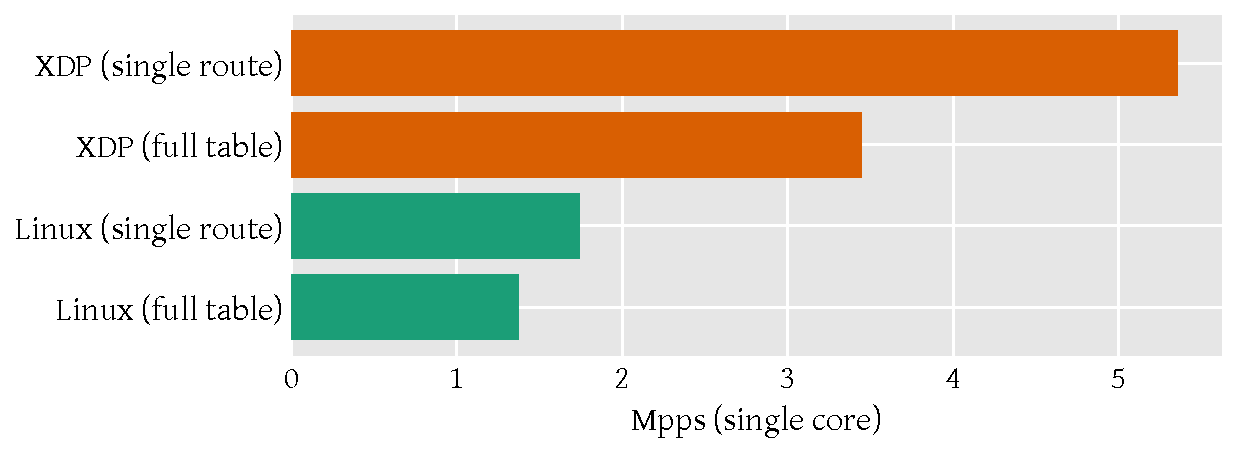
\includegraphics[width=0.95\textwidth,height=5cm]{original/router-fwd.pdf} % first figure itself
        \subcaption{In Original Paper}
        \label{graph:route:a}
    \end{minipage}\hfill
    
    \begin{minipage}{0.7\textwidth}
        \centering
        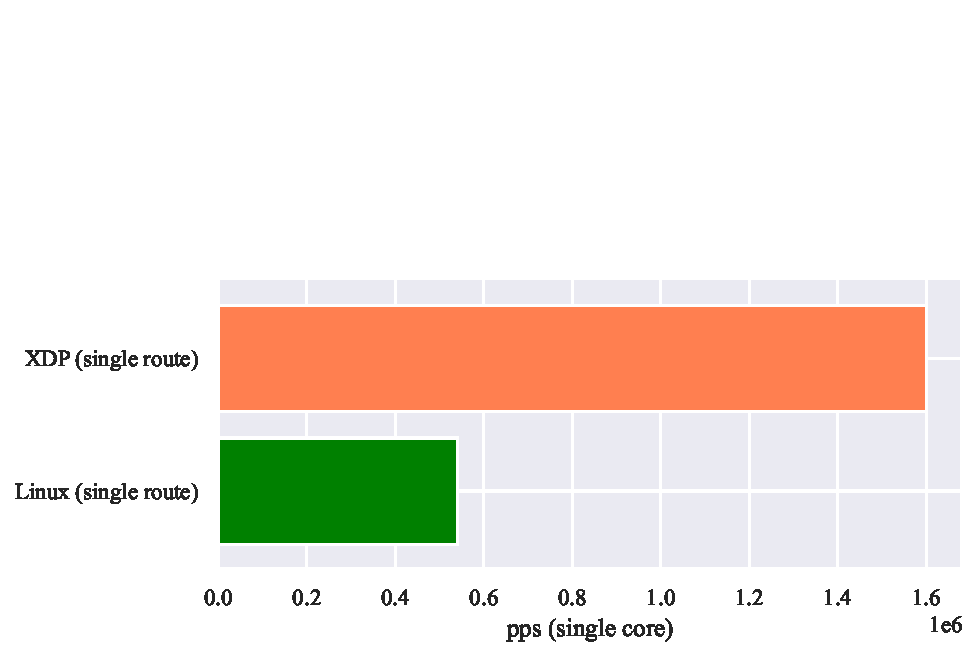
\includegraphics[width=0.95\textwidth,height=5cm]{img/router-fwd.pdf} % second figure itself
        \subcaption{In Our experiment}
        \label{graph:route:b}
    \end{minipage}
     \caption{Software routing performance. Since the performance scales linearly with the number of cores, only the results of a single core are shown.}
     \label{graph:route}
\end{figure}



\subsection{Inline DoS Mitigation}

DoS attacks are the most common attack that effect the internet. They also happen in the form of distributed attacks (DDoS attacks) from compromised devices. With XDP it is possible to deploy packet filtering to mitigate such attacks directly at the application server, without needing to change applications. 
For this test we used XDP program that parses the packet headers and perform small number of tests to indentify attack traffic and drop it. For measurement we used Netperf benchmarking tool \cite{netperf} which measures TCP based round-trip time, and outputs number of transactions per second. We run our experiment on a single core, then simulate DoS attack by offering an increasing load of small UDP packets matching the packet filter. We measure TCP transactions performance as attack traffic increases both with and without XDP filter installed.  

Figure~\ref{graph:ddos:b} compares the TCP performance with and without XDP protection. Without XDP filter, performance drops rapidly, being halved at 100kpps of attack traffic .However with XDP filter in place, the TCP transaction performance is stable at around 40,000 transactions per second. This shows that DDoS filtering is feasible to perform in XDP. Also our results are comparable to the original results shown in Figure ~\ref{graph:ddos:a} 

\begin{figure}
    \centering
    \begin{minipage}{0.49\textwidth}
        \centering
        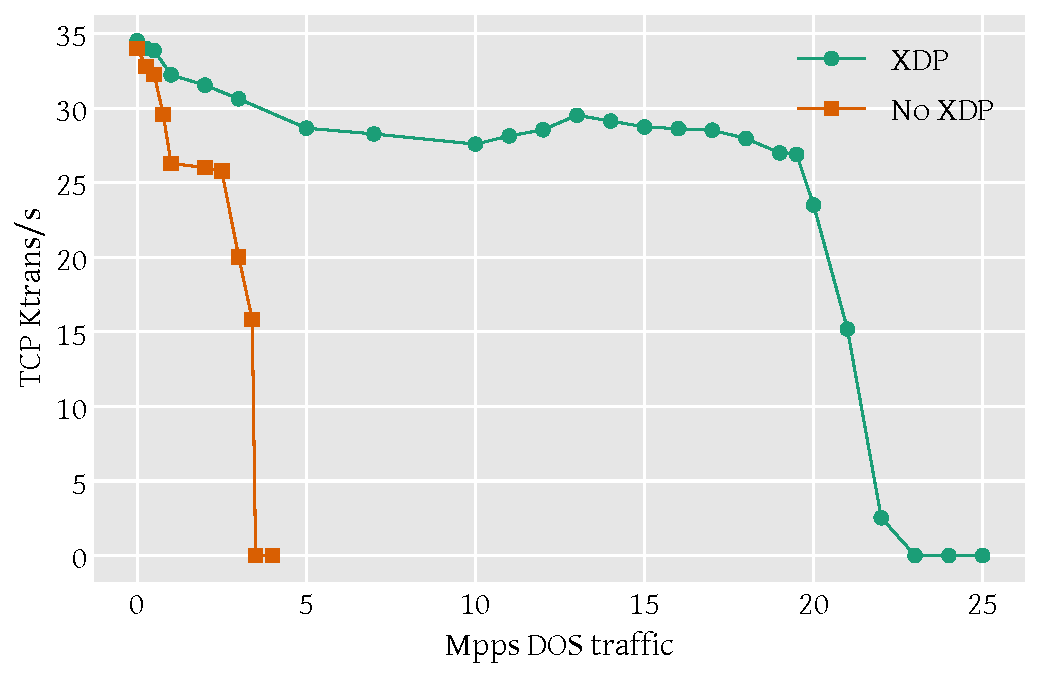
\includegraphics[width=0.95\textwidth,height=5.5cm]{original/ddos-test.pdf} % first figure itself
        \subcaption{throughput in Higher PPS}
        \label{graph:ddos:a}
    \end{minipage}\hfill
    \begin{minipage}{0.49\textwidth}
        \centering
        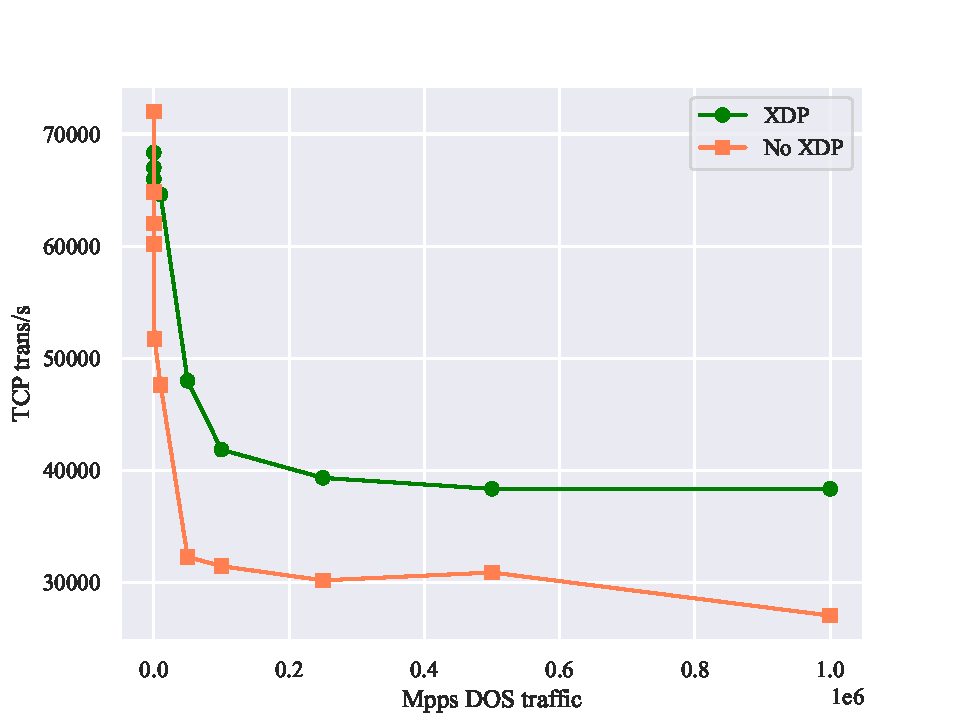
\includegraphics[width=0.95\textwidth,height=5.5cm]{img/dos-test.pdf} % second figure itself
        \subcaption{throughput in Lower PPS.}
        \label{graph:ddos:b}
    \end{minipage}
     \caption{DDoS performance. Number of TCP transactions per second as the level of attack traffic directed at the server increases}
     \label{graph:ddos}
\end{figure}


\section{Conclusion}

The experiments conducted showed that the XDP is faster than Linux network stack both in raw packet processing and couple of real-world use cases. Given that XDP is part of the Linux kernel, it undergoes continuous improvement. This means the XDP capabilities will only increases over time. XDP is a perfect solution which lies between kernel by-pass techniques and regular operating  system network stack. 

Getting benefits of Operating system capabilities  along with faster packet process power puts it a strong position to accelerate the transport protocols of the future and there has been some initial work on how XDP can improve QUIC protocol \cite{eQUIC}. While this is far from trivial, this presents an exciting opportunity for researchers to expand the scope of XDP system.

\vspace{4cm}

\begin{center}
    \textbf{Acknowledgements}
    \vspace{0.5cm}
    
    The Trellis Reading group discussions inspired me to read about fast packet processing technologies. Sincere thanks to Paul Lu for extending submission deadline, which gave time to  run these experiments in cloud environment.
    \begin{minipage}{0.8\linewidth}
    \end{minipage}
    \noindent\ignorespaces
\end{center}

\vspace{4cm}
%%%%%%%%%%%%%%%%%%%%%%%%
% Bibliography Begins Here %
%%%%%%%%%%%%%%%%%%%%%%%%


\begin{spacing}{1}
\bibliographystyle{plainnat}
\bibliography{xdp_report}
\end{spacing}

\end{document}
